% Options for packages loaded elsewhere
\PassOptionsToPackage{unicode}{hyperref}
\PassOptionsToPackage{hyphens}{url}
%
\documentclass[
]{article}
\usepackage{amsmath,amssymb}
\usepackage{lmodern}
\usepackage{iftex}
\ifPDFTeX
  \usepackage[T1]{fontenc}
  \usepackage[utf8]{inputenc}
  \usepackage{textcomp} % provide euro and other symbols
\else % if luatex or xetex
  \usepackage{unicode-math}
  \defaultfontfeatures{Scale=MatchLowercase}
  \defaultfontfeatures[\rmfamily]{Ligatures=TeX,Scale=1}
\fi
% Use upquote if available, for straight quotes in verbatim environments
\IfFileExists{upquote.sty}{\usepackage{upquote}}{}
\IfFileExists{microtype.sty}{% use microtype if available
  \usepackage[]{microtype}
  \UseMicrotypeSet[protrusion]{basicmath} % disable protrusion for tt fonts
}{}
\makeatletter
\@ifundefined{KOMAClassName}{% if non-KOMA class
  \IfFileExists{parskip.sty}{%
    \usepackage{parskip}
  }{% else
    \setlength{\parindent}{0pt}
    \setlength{\parskip}{6pt plus 2pt minus 1pt}}
}{% if KOMA class
  \KOMAoptions{parskip=half}}
\makeatother
\usepackage{xcolor}
\usepackage[margin=1in]{geometry}
\usepackage{color}
\usepackage{fancyvrb}
\newcommand{\VerbBar}{|}
\newcommand{\VERB}{\Verb[commandchars=\\\{\}]}
\DefineVerbatimEnvironment{Highlighting}{Verbatim}{commandchars=\\\{\}}
% Add ',fontsize=\small' for more characters per line
\usepackage{framed}
\definecolor{shadecolor}{RGB}{248,248,248}
\newenvironment{Shaded}{\begin{snugshade}}{\end{snugshade}}
\newcommand{\AlertTok}[1]{\textcolor[rgb]{0.94,0.16,0.16}{#1}}
\newcommand{\AnnotationTok}[1]{\textcolor[rgb]{0.56,0.35,0.01}{\textbf{\textit{#1}}}}
\newcommand{\AttributeTok}[1]{\textcolor[rgb]{0.77,0.63,0.00}{#1}}
\newcommand{\BaseNTok}[1]{\textcolor[rgb]{0.00,0.00,0.81}{#1}}
\newcommand{\BuiltInTok}[1]{#1}
\newcommand{\CharTok}[1]{\textcolor[rgb]{0.31,0.60,0.02}{#1}}
\newcommand{\CommentTok}[1]{\textcolor[rgb]{0.56,0.35,0.01}{\textit{#1}}}
\newcommand{\CommentVarTok}[1]{\textcolor[rgb]{0.56,0.35,0.01}{\textbf{\textit{#1}}}}
\newcommand{\ConstantTok}[1]{\textcolor[rgb]{0.00,0.00,0.00}{#1}}
\newcommand{\ControlFlowTok}[1]{\textcolor[rgb]{0.13,0.29,0.53}{\textbf{#1}}}
\newcommand{\DataTypeTok}[1]{\textcolor[rgb]{0.13,0.29,0.53}{#1}}
\newcommand{\DecValTok}[1]{\textcolor[rgb]{0.00,0.00,0.81}{#1}}
\newcommand{\DocumentationTok}[1]{\textcolor[rgb]{0.56,0.35,0.01}{\textbf{\textit{#1}}}}
\newcommand{\ErrorTok}[1]{\textcolor[rgb]{0.64,0.00,0.00}{\textbf{#1}}}
\newcommand{\ExtensionTok}[1]{#1}
\newcommand{\FloatTok}[1]{\textcolor[rgb]{0.00,0.00,0.81}{#1}}
\newcommand{\FunctionTok}[1]{\textcolor[rgb]{0.00,0.00,0.00}{#1}}
\newcommand{\ImportTok}[1]{#1}
\newcommand{\InformationTok}[1]{\textcolor[rgb]{0.56,0.35,0.01}{\textbf{\textit{#1}}}}
\newcommand{\KeywordTok}[1]{\textcolor[rgb]{0.13,0.29,0.53}{\textbf{#1}}}
\newcommand{\NormalTok}[1]{#1}
\newcommand{\OperatorTok}[1]{\textcolor[rgb]{0.81,0.36,0.00}{\textbf{#1}}}
\newcommand{\OtherTok}[1]{\textcolor[rgb]{0.56,0.35,0.01}{#1}}
\newcommand{\PreprocessorTok}[1]{\textcolor[rgb]{0.56,0.35,0.01}{\textit{#1}}}
\newcommand{\RegionMarkerTok}[1]{#1}
\newcommand{\SpecialCharTok}[1]{\textcolor[rgb]{0.00,0.00,0.00}{#1}}
\newcommand{\SpecialStringTok}[1]{\textcolor[rgb]{0.31,0.60,0.02}{#1}}
\newcommand{\StringTok}[1]{\textcolor[rgb]{0.31,0.60,0.02}{#1}}
\newcommand{\VariableTok}[1]{\textcolor[rgb]{0.00,0.00,0.00}{#1}}
\newcommand{\VerbatimStringTok}[1]{\textcolor[rgb]{0.31,0.60,0.02}{#1}}
\newcommand{\WarningTok}[1]{\textcolor[rgb]{0.56,0.35,0.01}{\textbf{\textit{#1}}}}
\usepackage{graphicx}
\makeatletter
\def\maxwidth{\ifdim\Gin@nat@width>\linewidth\linewidth\else\Gin@nat@width\fi}
\def\maxheight{\ifdim\Gin@nat@height>\textheight\textheight\else\Gin@nat@height\fi}
\makeatother
% Scale images if necessary, so that they will not overflow the page
% margins by default, and it is still possible to overwrite the defaults
% using explicit options in \includegraphics[width, height, ...]{}
\setkeys{Gin}{width=\maxwidth,height=\maxheight,keepaspectratio}
% Set default figure placement to htbp
\makeatletter
\def\fps@figure{htbp}
\makeatother
\setlength{\emergencystretch}{3em} % prevent overfull lines
\providecommand{\tightlist}{%
  \setlength{\itemsep}{0pt}\setlength{\parskip}{0pt}}
\setcounter{secnumdepth}{-\maxdimen} % remove section numbering
\usepackage{xeCJK}
\ifLuaTeX
  \usepackage{selnolig}  % disable illegal ligatures
\fi
\IfFileExists{bookmark.sty}{\usepackage{bookmark}}{\usepackage{hyperref}}
\IfFileExists{xurl.sty}{\usepackage{xurl}}{} % add URL line breaks if available
\urlstyle{same} % disable monospaced font for URLs
\hypersetup{
  hidelinks,
  pdfcreator={LaTeX via pandoc}}

\author{}
\date{\vspace{-2.5em}}

\begin{document}

\hypertarget{biostatistics-homework-4}{%
\section{Biostatistics Homework 4}\label{biostatistics-homework-4}}

By \(\mathbb{L}\)umi (张鹿鸣12112618)

\vspace{5mm}

\hypertarget{gene-expression-distribution}{%
\subsection{1 Gene Expression
Distribution}\label{gene-expression-distribution}}

\hypertarget{section}{%
\subsubsection{1.1)}\label{section}}

\begin{Shaded}
\begin{Highlighting}[]
\FunctionTok{curve}\NormalTok{(}\FunctionTok{dgamma}\NormalTok{(x, }\AttributeTok{shape =} \DecValTok{2}\NormalTok{, }\AttributeTok{scale =} \DecValTok{1}\NormalTok{) }\SpecialCharTok{+} \FunctionTok{dnorm}\NormalTok{(x, }\AttributeTok{mean =} \DecValTok{7}\NormalTok{, }\AttributeTok{sd =} \FloatTok{0.5}\NormalTok{) }\SpecialCharTok{/} \DecValTok{20}\NormalTok{,}
      \AttributeTok{from =} \DecValTok{0}\NormalTok{, }\AttributeTok{to =} \DecValTok{10}\NormalTok{,}
      \AttributeTok{main =} \StringTok{"Gene Expression Distribution"}\NormalTok{,}
      \AttributeTok{xlab =} \StringTok{"Gene expression level"}\NormalTok{, }\AttributeTok{ylab =} \StringTok{"Counts"}\NormalTok{,}
      \AttributeTok{xaxt =} \StringTok{\textquotesingle{}n\textquotesingle{}}\NormalTok{, }\AttributeTok{yaxt =} \StringTok{\textquotesingle{}n\textquotesingle{}}\NormalTok{)}
\end{Highlighting}
\end{Shaded}

\begin{center}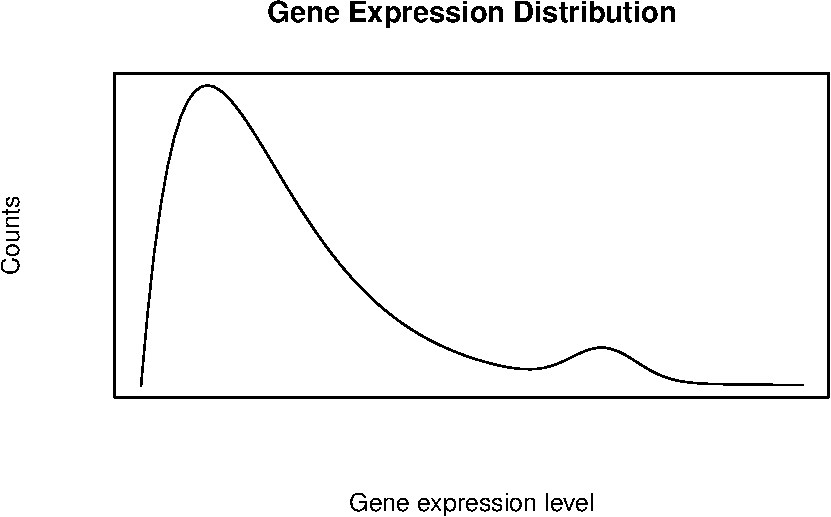
\includegraphics{hw4_files/figure-latex/unnamed-chunk-1-1} \end{center}

I think the gene expression pattern will follow a Gamma distribution,
which in other words is a distribution skewed to the right. Because many
genes are not significantly expressed, thus most of the genes will have
a rather low expression level. But some genes are expressed in a very
significant amount, because they might be essential for cell survival,
or are the signatures for this specific cell type. So a few counts will
lie in the high expression area. Thus I think a Gamma distribution with
a small bump on the right will fit best.

\hypertarget{section-1}{%
\subsubsection{1.2)}\label{section-1}}

\begin{Shaded}
\begin{Highlighting}[]
\FunctionTok{curve}\NormalTok{(}\FunctionTok{dnorm}\NormalTok{(x, }\AttributeTok{mean =} \DecValTok{0}\NormalTok{, }\AttributeTok{sd =} \DecValTok{1}\NormalTok{), }
      \AttributeTok{from =} \SpecialCharTok{{-}}\DecValTok{4}\NormalTok{, }\AttributeTok{to =} \DecValTok{4}\NormalTok{,}
      \AttributeTok{main =} \StringTok{"Normal Distribution"}\NormalTok{,}
      \AttributeTok{xlab =} \StringTok{"Gene expression level"}\NormalTok{, }\AttributeTok{ylab =} \StringTok{"Cell counts"}\NormalTok{,}
      \AttributeTok{xaxt =} \StringTok{\textquotesingle{}n\textquotesingle{}}\NormalTok{, }\AttributeTok{yaxt =} \StringTok{\textquotesingle{}n\textquotesingle{}}\NormalTok{)}
\end{Highlighting}
\end{Shaded}

\begin{center}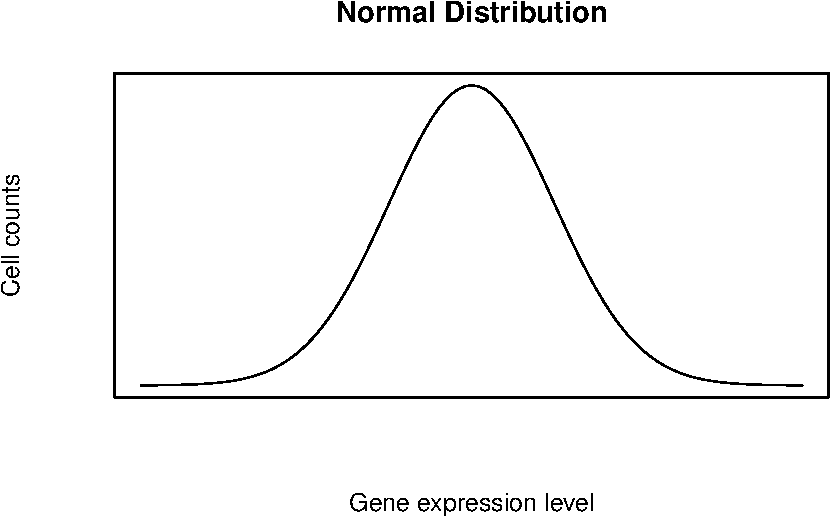
\includegraphics{hw4_files/figure-latex/unnamed-chunk-2-1} \end{center}

I think the \emph{Nanog} gene expression across the embryonic stem cell
population should follow a normal distribution. Because they are all
from the same embryonic stem cell population, their expression of a
particular gene should not vary from a certain value vary dramatically,
although there might be fluctuations.

\hypertarget{section-2}{%
\subsubsection{1.3)}\label{section-2}}

I think the distributions of 1.1) and 1.2) are not the same. 1.1) is the
distribution of expression levels of all the genes in a single cell, it
shows that genes are expressed differently in this cell. 1.2) is the
distribution of the expression of a gene in multiple cells, it shows the
general level of expression of this gene in all the cells.

\hypertarget{weaver-ants}{%
\subsection{2. Weaver ants}\label{weaver-ants}}

\hypertarget{section-3}{%
\subsubsection{2.1)}\label{section-3}}

\begin{Shaded}
\begin{Highlighting}[]
\FunctionTok{curve}\NormalTok{(}\FunctionTok{dnorm}\NormalTok{(x, }\AttributeTok{mean =} \DecValTok{5}\NormalTok{, }\AttributeTok{sd =} \FloatTok{1.7}\NormalTok{) }\SpecialCharTok{+} \FunctionTok{dnorm}\NormalTok{(x, }\AttributeTok{mean =} \DecValTok{10}\NormalTok{, }\AttributeTok{sd =} \FloatTok{1.6}\NormalTok{),}
      \AttributeTok{from =} \DecValTok{0}\NormalTok{, }\AttributeTok{to =} \DecValTok{14}\NormalTok{,}
      \AttributeTok{main =} \StringTok{\textquotesingle{}Population Distribution of Weaver Ants Body Length\textquotesingle{}}\NormalTok{,}
      \AttributeTok{xlab =} \StringTok{\textquotesingle{}Weaver Ant Body Length (mm)\textquotesingle{}}\NormalTok{,}
      \AttributeTok{yaxt =} \StringTok{\textquotesingle{}n\textquotesingle{}}\NormalTok{, }\AttributeTok{ylab =} \StringTok{\textquotesingle{}Counts\textquotesingle{}}\NormalTok{)}
\end{Highlighting}
\end{Shaded}

\begin{center}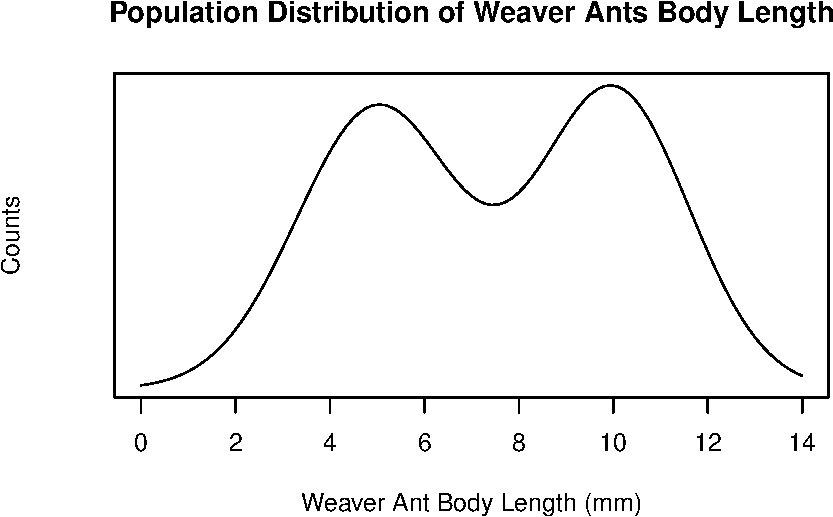
\includegraphics{hw4_files/figure-latex/unnamed-chunk-3-1} \end{center}

Because there are two types of weaver ants with different body lengths,
I suspect that the curve can have two peaks accounting for the two
different types of ants. Among the two different types of ants, the body
length should follow a normal distribution respectively, so the
population distribution of the body length should simply be the addition
of the two normal distributions.

\hypertarget{section-4}{%
\subsubsection{2.2)}\label{section-4}}

Since the sample is drawn randomly from the population, we can assume
that the sample follows the same type of distribution of the population.

\begin{Shaded}
\begin{Highlighting}[]
\FunctionTok{hist}\NormalTok{(}\FunctionTok{rnorm}\NormalTok{(}\DecValTok{312}\NormalTok{, }\AttributeTok{mean =} \DecValTok{5}\NormalTok{, }\AttributeTok{sd =} \FloatTok{1.7}\NormalTok{) }\SpecialCharTok{+} \FunctionTok{rnorm}\NormalTok{(}\DecValTok{313}\NormalTok{, }\AttributeTok{mean =} \DecValTok{10}\NormalTok{, }\AttributeTok{sd =} \FloatTok{1.6}\NormalTok{),}
     \AttributeTok{main =} \StringTok{\textquotesingle{}Sample Distribution of Weaver Ants Body Length\textquotesingle{}}\NormalTok{,}
     \AttributeTok{xlab =} \StringTok{\textquotesingle{}Weaver Ant Body Length (mm)\textquotesingle{}}\NormalTok{, }\AttributeTok{xaxt =} \StringTok{\textquotesingle{}n\textquotesingle{}}\NormalTok{,}
     \AttributeTok{yaxt =} \StringTok{\textquotesingle{}n\textquotesingle{}}\NormalTok{, }\AttributeTok{ylab =} \StringTok{\textquotesingle{}Counts\textquotesingle{}}\NormalTok{,}
     \AttributeTok{breaks =} \DecValTok{50}\NormalTok{)}
\end{Highlighting}
\end{Shaded}

\begin{verbatim}
## Warning in rnorm(312, mean = 5, sd = 1.7) + rnorm(313, mean = 10, sd = 1.6):
## longer object length is not a multiple of shorter object length
\end{verbatim}

\begin{center}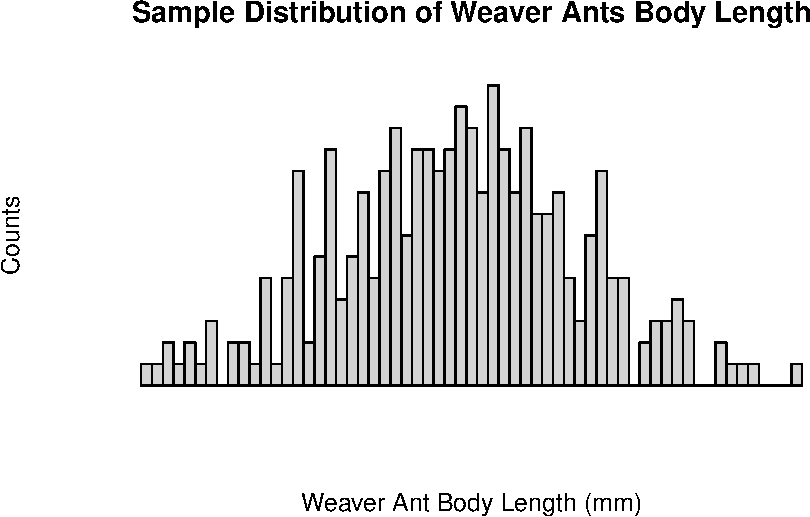
\includegraphics{hw4_files/figure-latex/unnamed-chunk-4-1} \end{center}

\hypertarget{section-5}{%
\subsubsection{2.3)}\label{section-5}}

When you randomly choose multiple groups of 625 weaver ants, the mean
body length should follow a normal distribution with
\(\mu = 7, \sigma^2 = (\frac{10}{25})^2\). Suppose \(X_i\) is the random
variable indicating the mean body length for the 625 weaver ants.

\[
P(X_i \leq 7.5) = P(Z \leq \frac{7.5 - \mu}{\sigma}) = P(Z \leq 1.25) \approx 0.8944
\]

So the probability of getting a mean from 625 weaver ants that is
smaller than 7.5mm is 0.8944.

\hypertarget{a-simple-random-sample}{%
\subsection{3 A Simple Random Sample}\label{a-simple-random-sample}}

C

\hypertarget{the-concept-of-population}{%
\subsection{4 The Concept of
Population}\label{the-concept-of-population}}

{[} tick {]} It is better to think of our population as an abstract
concept.

{[} tick {]} The population is effectively infinite.

\hypertarget{a-practical-simple-random-sampling-strategy}{%
\subsection{5 A Practical Simple Random Sampling
Strategy}\label{a-practical-simple-random-sampling-strategy}}

\begin{Shaded}
\begin{Highlighting}[]
\FunctionTok{sample}\NormalTok{(}\DecValTok{1}\SpecialCharTok{:}\DecValTok{1000}\NormalTok{, }\DecValTok{20}\NormalTok{)}
\end{Highlighting}
\end{Shaded}

\begin{verbatim}
##  [1] 543 834 491 485 269 681 249 178 247 212  31 910 798 516 902 476 890 972 815
## [20] 494
\end{verbatim}

But actually, I think just taking the first 20 participants is OK, if
your 1000 participants are labeled randomly.

\hypertarget{triceps-skinfold-thickness}{%
\subsection{6 Triceps skinfold
thickness}\label{triceps-skinfold-thickness}}

\hypertarget{section-6}{%
\subsubsection{6.1)}\label{section-6}}

Similar to problem 2 about the ants, suppose the mean triceps skinfold
thickness of 25 people follows is the random variable \(X\). Than \(X\)
should follow a normal distribution with parameters
\(\mu = 1.35, \sigma^2 = 0.01\).

\[
P(X \leq 1.05) = P(Z \leq \frac{1.05 - \mu}{0.1} )  = P(Z \leq -3) \approx 0.0013
\]

\hypertarget{section-7}{%
\subsubsection{6.2)}\label{section-7}}

From 6.1) we can see that, getting 25 random people and observing a mean
value smaller than 1.05 is very rare ( \(p < 0.0013\) ). From the
possibility, you can say that it's a once in a thousand opportunity to
get a random sample like this. We can also calculate the possibility to
observe a mean larger than \$X = 0.92\$, which is \(p = 0.99999\). It is
highly unlikely to get a value smaller than 0.92cm. Thus we can say that
these people who suffer from COPD are significantly different from the
normal population.

\hypertarget{decrease-manufacturing-variability}{%
\subsection{7 Decrease Manufacturing
Variability}\label{decrease-manufacturing-variability}}

\hypertarget{section-8}{%
\subsubsection{7.1)}\label{section-8}}

Suppose that the weights of bags of potato chips follows the random
variable \(X\).

\[
P(X \leq 330) = P(Z \leq \frac{330 - 362}{20} ) = P( Z\leq -1.6) \approx 0.0548
\]

\hypertarget{section-9}{%
\subsubsection{7.2)}\label{section-9}}

Suppose the random variable \(Y\) describes the mean of the sample with
size 100. \(Y\) follows a normal distribution \(Y \sim N(362, 4)\).

\[
P(360 < Y < 363) = P( -1 < Z < 0.5) = 0.5328
\]

\hypertarget{section-10}{%
\subsubsection{7.3)}\label{section-10}}

Because only 1\% of bags weigh less than 330g, the Z score for 1\% is
\(-2.326\).

\[
\begin{aligned}
\frac{330 - 362}{\sigma} &= -2.326 \\
\sigma &\approx 13.75
\end{aligned}
\]

\hypertarget{a-hypothetical-linear-pdf}{%
\subsection{8 A Hypothetical Linear
PDF}\label{a-hypothetical-linear-pdf}}

\hypertarget{section-11}{%
\subsubsection{8.1)}\label{section-11}}

\[
\begin{aligned}
\int_0^1 (1 - \theta) + 2\theta x dx = [(1-\theta)x + \theta x^2 ]_0^1 = 1
\end{aligned}
\]

This shows that the area under the PDF is 1.

\[
\begin{aligned}
0 < &x<1 \\
1- \theta < &f_\mathbf{X}(x) < 1 + \theta
\end{aligned}
\]

Because \(-1 < \theta < 1\), \(0 < f_\mathbf{X}(x) < 2\).

So this probability density functions fulfills the basic properties of
the PDF. That is, the area under the curve is 1, and all the density
values are larger than 0.

\hypertarget{section-12}{%
\subsubsection{8.2)}\label{section-12}}

\[
F_X(x) = \int_0^x(1-\theta) + 2\theta t dt = (1-\theta)x + \theta x^2
\]

So

\[
F_X(x) = \begin{cases}
1 &, x > 1 \\
(1-\theta) x + \theta x^2 &, 1 > x > 0 \\
0 &, x\leq0
\end{cases}
\]

\hypertarget{section-13}{%
\subsubsection{8.3)}\label{section-13}}

\[
\begin{aligned}
E(X) &= \int_0^1 x(1-\theta) + 2\theta x^2 dx \\
&= \frac{(1-\theta)x^2}{2} + \frac{2\theta x^3}{3} \rbrack_0^1 \\
& = \frac{3 + \theta}{6}
\end{aligned}
\]

\hypertarget{section-14}{%
\subsubsection{8.4)}\label{section-14}}

\[
\mathcal L(\theta; x_1,x_2, ..., x_n) = \prod_{i=1}^n [(1-\theta) + 2\theta x_i]
\]

So, \(\ell(\theta;x) = \ln{\mathcal L(\theta; x)}\)

\[
\ell (\theta; x) = \sum_{i=1}^n\ln{[(1-\theta) + 2\theta x_i]}
\]

\hypertarget{section-15}{%
\subsubsection{8.5)}\label{section-15}}

\[
\begin{aligned}
\frac{d \ell}{d \theta} = \sum_{i=1}^n \frac{2x_i - 1}{(1-\theta) + 2\theta x_i} = 0 \\
\hat{\theta} = t \\
\sum_{i=1}^n \frac{2x_i - 1}{(1-\hat \theta) + 2\hat \theta x_i}= \sum_{i=1}^n \frac{2x_i - 1}{(1-t) + 2t x_i} = 0
\end{aligned}
\]

So we choose B.

\hypertarget{waiting-time-between-text-messages}{%
\subsection{9 Waiting Time Between Text
Messages}\label{waiting-time-between-text-messages}}

\[
\begin{aligned}
\mathcal{L}(\lambda; x) &= \prod_{i=1}^n\lambda e^{-\lambda x_i} = \lambda^n e^{-\lambda \sum_{i=1}^nx_i} \\
\ell (\lambda;x) &= \ln{\mathcal{L}(\lambda;x)} \\
&= n \ln \lambda - \lambda \sum_{i=1}^n x_i \\
\frac{d \ell}{d \lambda} &= 0 = \frac{n}{\hat \lambda}- \sum_{i=1}^n x_i \\
\hat \lambda &= \frac{n}{\sum_{i=1}^n x_i}
\end{aligned}
\]

So the maximum likelihood estimation of \(\lambda\) is
\(\frac{n}{\sum_{i=1}^n x_i}\).

\end{document}
